\chapter{Implementación}
\label{chapter:5-Implementación}
En esta sección se detallan las distintas tecnologías, herramientas y software de terceros que se utilizaron. Se describe precisamente como, donde utilizamos dichas tecnologías y el porqué se eligieron. 

\section{Tecnologías y Lenguajes}
\label{section:5-Tecnologías y Lenguajes}

Se detallarán las tecnologías utilizada en esta sección. Tanto en el proceso de desarrollo como en el producto final publicado. Cabe destacar que optamos por utilizar unicamente código abierto (Open Source) y gratis. Esto se decidió por dos objetivos en mente, el objetivo de que el producto pueda ser mantenible por el futuro sin ningún tipo impedimentos de costo y con el objetivo de utilizar herramientas populares con un gran numero de desarrolladores aptos en estas tecnologías.

En esta sección se detallan las tecnologías empleadas tanto en el proceso de desarrollo como en el producto final publicado. Es importante destacar que se optó por utilizar exclusivamente tecnologías de código abierto (Open Source) y gratuitas. Esta decisión es debido a dos objetivos fundamentales:
En primer lugar, garantizar que el producto sea mantenible y sostenible en el futuro sin impedimentos económicos que comprometan la continuidad del proyecto; 
En segundo lugar, aprovechar herramientas populares, ampliamente adoptadas y por un buen numero de desarrolladores. Asegurando la disponibilidad de una base extensa de desarrolladores capacitados en estas tecnologías y facilita la incorporación de nuevos colaboradores al proyecto.

\subsection[Frontend]{\Gls{frontend}}
\label{subsection:5-frontend}
Aquí nos expandimos acerca de las tecnologías utilizadas del lado cliente.
\begin{itemize}
\item \textbf{\Gls{react}}: Biblioteca de JavaScript para construir interfaces de usuario interactivas. \Gls{react} es código abierto y es de los frameworks más apreciados, con un de 74,5\% de apreciación según \cite{React_JS_Coderhouse}. \Gls{react} destaca en rendimiento y agiliza la velocidad de desarrollo.
\item \textbf{TypeScript}: Añade tipado estático a Javascript. Facilita la detección de errores durante el desarrollo. Añade interfaces y clases, agilizando el desarrollo.
\item \textbf{TailwindCSS}: Framework de CSS. Permite personalizar la interfaz de usuario fácilmente sin necesidad de crear archivos archivos css aparte para definir clases. 
\item \textbf{\acrshort{json} Web \Gls{token} (JWT)}:
Estándar para autenticación en aplicaciones web. Permite transmitir información de usuario de forma segura desde el lado cliente a el servidor. Esto se muesta en la figura \autoref{fig:JWT}

\begin{figure}[htbp]
    \centering
    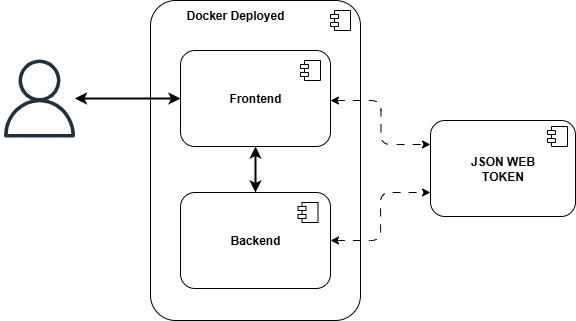
\includegraphics[width=\linewidth]{Nuestro/Imagenes/Arquitectura/JSW.drawio.png}
    
    \caption{Diagrama de Funcionalidad de \acrshort{json}Web \Gls{token}}
    \label{fig:JWT}
\end{figure}
\end{itemize}

\subsection{Entorno}
\label{subsection:5-Entorno}
\begin{itemize}
    \item \textbf{Docker}: Plataforma de contenedorización que empaqueta aplicaciones y sus dependencias en contenedores aislados. Garantiza que el software funcione de manera consistente en cualquier entorno, desde desarrollo hasta producción.
    \item \textbf{uvicorn}: Gestor de paquetes y entornos virtuales para Python extremadamente rápido, escrito en Rust. Sirve como reemplazo moderno de pip y venv, acelerando significativamente la instalación de dependencias.
\end{itemize}
\subsection[Backend]{\Gls{backend}}
\label{subsection:5-backend}
\begin{itemize}
    \item \textbf{Python}: Lenguaje de programación interpretado, de alto nivel y multipropósito. Es conocido por su sintaxis clara y legible, y es ampliamente utilizado en desarrollo web, ciencia de datos y automatización.
    \item \textbf{FastAPI}: Framework web moderno para Python que permite crear APIs REST de alto rendimiento. Incluye validación automática de datos, documentación interactiva generada automáticamente y soporte nativo para operaciones asíncronas.
\end{itemize}

\subsection{Base de Datos}
\label{subsection:5-Base de Datos}
\begin{itemize}
    \item \textbf{PostgreSQL}: Sistema de gestión de bases de datos relacionales de código abierto, robusto y con soporte para características avanzadas como transacciones ACID, índices complejos y extensiones personalizadas.
    \item \textbf{PGVector}: Extensión de PostgreSQL que añade soporte para almacenar y consultar vectores de embeddings. Permite realizar búsquedas de similitud semántica, fundamental para aplicaciones de inteligencia artificial y búsqueda vectorial.

\end{itemize}

LangChain:
Framework de desarrollo para aplicaciones con LLMs. Proporciona abstracciones modulares (chains, agents, memory) que facilitan la orquestación de prompts, integración con APIs externas, gestión de \gls{contexto} conversacional y construcción de pipelines complejos mediante componentes reutilizables y composables.
Multilingual Embeddings:
Representaciones vectoriales que mapean texto de múltiples idiomas a un espacio semántico compartido. Permiten comparación cross-lingual y transferencia de conocimiento entre lenguas mediante técnicas como alineación de espacios vectoriales o entrenamiento con corpus paralelos.
\subsection{Transcriber}
\label{subsection:5-1-Transcriber}
\begin{itemize}
    \item {Whisper}
\end{itemize}
\subsection{LLM}
\label{subsection:5-LLM}
LLM


\todo[inline,color=cyan]{Aca pensamos dejar estadiscticas de las herramientas}
\begin{itemize}
\item \textbf{Mistral}:
Familia de modelos de lenguaje de código abierto desarrollados por Mistral AI. Destacan por su eficiencia computacional mediante arquitecturas optimizadas (Grouped-Query Attention, Sliding Window Attention) que logran rendimiento competitivo con modelos más grandes, manteniendo menores requisitos de hardware y latencia reducida.
\item \textbf{LangChain}:
Framework de desarrollo para aplicaciones con LLMs. Proporciona abstracciones modulares (chains, agents, memory) que facilitan la orquestación de prompts, integración con APIs externas, gestión de \gls{contexto} conversacional y construcción de pipelines complejos mediante componentes reutilizables y composables.
\item \textbf{Multilingual Embeddings}:
Representaciones vectoriales que mapean texto de múltiples idiomas a un espacio semántico compartido. Permiten comparación cross-lingual y transferencia de conocimiento entre lenguas mediante técnicas como alineación de espacios vectoriales o entrenamiento con corpus paralelos.
    
\end{itemize}

FastAPI: Proporciona los endpoints \acrshort{http} para exponer los servicios del LLM, permitiendo la integración de modelos de inteligencia artificial en la arquitectura mediante APIs eficientes y bien documentadas.

